\section{Discussion and results}

Both fjord models are run twice. The first run applies the original tidal forcing and the second run applies the adjusted tidal forcing. Nine major tidal constituents of diurnal (K$_1$, P$_1$, and O$_1$), semi diurnal (S$_2$, M$_2$, and N$_2$), and quarter diurnal (MN$_4$, M$_4$, and MS$_4$) frequencies are evaluated using harmonic analyses on the observed and modelled time series from both runs. The results improved for both the Oslofjord and for the Saltfjord. 

In the first run with the Oslofjord model, the modelled amplitudes did not match the observed amplitudes and the maxima appeared too late in time (Fig.~\ref{fig:Viker_timeseries}). In the second, run both phases and amplitudes improved. Table~\ref{tab:Viker} shows that the adjustments had the desired effect close to the open boundary. Notice the adjustment factors. The amplitudes of the principal lunar semidiurnal constituent (M$_2$) and its shallow water overtide (M$_4$) are increased, while the remaining are reduced. The size of these factors emphasize the need for adjustment of the tidal forcing. 
The modelled tides in the inner domain depend not only on the tidal forcing, but also on how the propagation of the tidal waves are represented in the model. Table~\ref{tab:Oscarsborg} shows that the modelled tides have improved also in the inner parts of the fjord. The remaining  discrepancies in the diurnal and quarter diurnal indicate challenges that might be caused by the representation of the propagation.

For the Saltfjord, time series reveal that the amplitudes are too small and the maxima appeared too early (Fig.~\ref{fig:Saltstraumen_timeseries}). Table~\ref{tab:Bodo} shows that the amplitudes are still too small in the second run, but closer to the observed values than in the first run. The error in phase for M$_2$ was only $0.8$ degrees which corresponds to three minutes (Table~\ref{tab:Bodo}). Again, the size of the adjustment factors emphasize the need for adjustment of the tidal forcing due to poor representation of the constituents in the original forcing. 

The barotropic tide propagates with a phase speed of $c = \omega/k \approx \sqrt{g h_c}$ where $g$ is the acceleration of gravity and $h_c$ is the characteristic depth. The distance from Viker to Oscarsborg is approximately 75 km and the mean depth is around 200 meters which gives an approximate phase speed of 44 m/s and a phase lag of approximately 28 minutes. According to Table~\ref{tab:Viker} and~\ref{tab:Oscarsborg} the observed phase lag is 17 degrees for M$_2$ which corresponds to 35 minutes which is only slightly longer than the approximate theoretical phase lag. 

Fields of the amplitude and phase for M$_2$ in the Oslofjord reveal some interesting phenomenons. Fig.~\ref{fig:Oslofjord_tidal_fields} shows fields of the resulting M$_2$ amplitudes and phases once the boundary forcing is corrected. 
The M$_2$ amplitude increases gradually northward from the open boundary in the south and all the way to the head of the fjord in the eastern branch. 
This can be explained by a progressive wave that propagates into the fjord and is reflected at the head.
The sum of two progressive waves gives a wave with increasing amplitude in the northward direction, as observed. 
Although the representation of M$_2$ at the boundary is in good agreement with the observations, the representation at the innermost stations deteriorates.
%The observed phase lag in the western branch is more pronounced in the observations than in the model. The cause is most probably the smoothing of the topography in the model.
In the western branch of the Oslofjord tidal choking occurs as water pass through the very narrow passage at the Svelvikstraum. Tidal chocking implies a decrease of tidal amplitude and a corresponding phase lag \cite[]{stigebrandt80} and occurs when the tidal wave enters a semi-enclosed basin through a sufficiently narrow inlet. This well-known phenomena is observed in several landlocked fjords and basins, for example Nord{\aa}svatnet and Saltfjord in Norway \cite[]{glenne63,eliassen01}, Mundau-Manguaba in Brazil \cite[]{oliveira93}, and Negembo Lagoon in Sri Lanka \cite[]{rydberg96}. 

The spatial variation is larger in the Saltfjord model as the choking is more pronounced (Fig.~\ref{fig:Saltstraumen_field}). Outside the Saltstraum, the narrow strait separating the two fjords, the M$_2$ amplitude is quite uniform at approximately $80$ cm, while on the inside it is only about $35$ cm. The corresponding phase delay is approximately $60$ degrees. Unfortunately, there is no available tidal gauges inside of the Saltstraum, but according to The Norwegian Hydrological Survey \cite[]{tide16} the M$_2$ amplitude in the Skjerstadfjord is 52.9 cm and the phase delay is 55 degrees compared with the sea level at Bod{\o}.
According to these records, the choking effect is slightly too strong in the model.
%, so we have no means of validating whether or not these values are correct. But we can speculate that we would se similar inconsistencies as those in the Oslofjord, due to smoothing of the model topography.

In coastal areas the currents vary both in time and over relatively short distances both vertically and horizontally. The currents at a position near Filtvedt in the Oslofjord were measured using a bottom-mounted profiling current meter from 18 September to 25 November 2014. The depth at the observation location was 167 meters. Time series of the observations reveal that the observed currents vary strongly with depth (Fig.~\ref{fig:Filtvedt_timeseries_obs}). The tides are evident except during storm surges where other effects dominate. In the lower levels more water run northwards during low and rising tide than southwards during high and descending tide. The tides in the upper levels are delayed in time compared to the lower levels. The velocities in the upper levels are difficult to determine due to noise. 

In order to compare observed and modelled tidal currents, harmonic analyses are performed on the depth averaged currents using T\_Tide. Time series of the observed and modelled tidal currents are constructed based on the calculated tidal components for the time period of the observations (Fig.~\ref{fig:Filtvedt_timeseries}). The time series reveal that the amplitudes in run 1 are too strong compared to the observations. 
An accurate representation of the currents at one specific position in shallow areas cannot be expected due to spatiotemporal challenges, but the tidal representation have improved after the adjustment (Table~\ref{tab:Filtvedt}). %Local features such as eddies seem to have a large impact on the phases.
%The  probability density functions reveal that the flow pattern has changed remarkable from run 1 to run 2 (Fig.~\ref{fig:Filtvedt_pdf}). 
%The currents below 40 meters depth are more evenly distributed in the model.  

The simple approach to adjust the tidal forcing gives improved and adequate accurate results for the two areas in question. 

%The Saltstraumen is one of the worlds strongest tidal currents. Due to a narrow passage the tidal amplitude is much smaller inside the narrow passage than outside the passage, resulting in strong currents. 
%The presence of Saltstraumen as a major impact on the circulation in the Saltfjord. According to \cite{svendsen96} an anticyclonic vortex is formed to the northeast of Saltstraumen, and a cyclonic vortex to the northwest.
%%% Fra Svendsen et. al 1996
%%%They are caused by the high velocity water coming out from Saltstraumen on the falling tide, where the velocity reaches a maximum of about 4 m s1: The anti-cyclonic vortex is weaker when the tide is rising, but does not reverse direction. The cyclonic vortex almost vanishes on rising tides. These results are in accordance with the results from Resipientunderskelse (Anon., 1990) where a direct measurement of the velocity field was performed over a time period of 10 days.


\begin{figure}[!t]
\centering
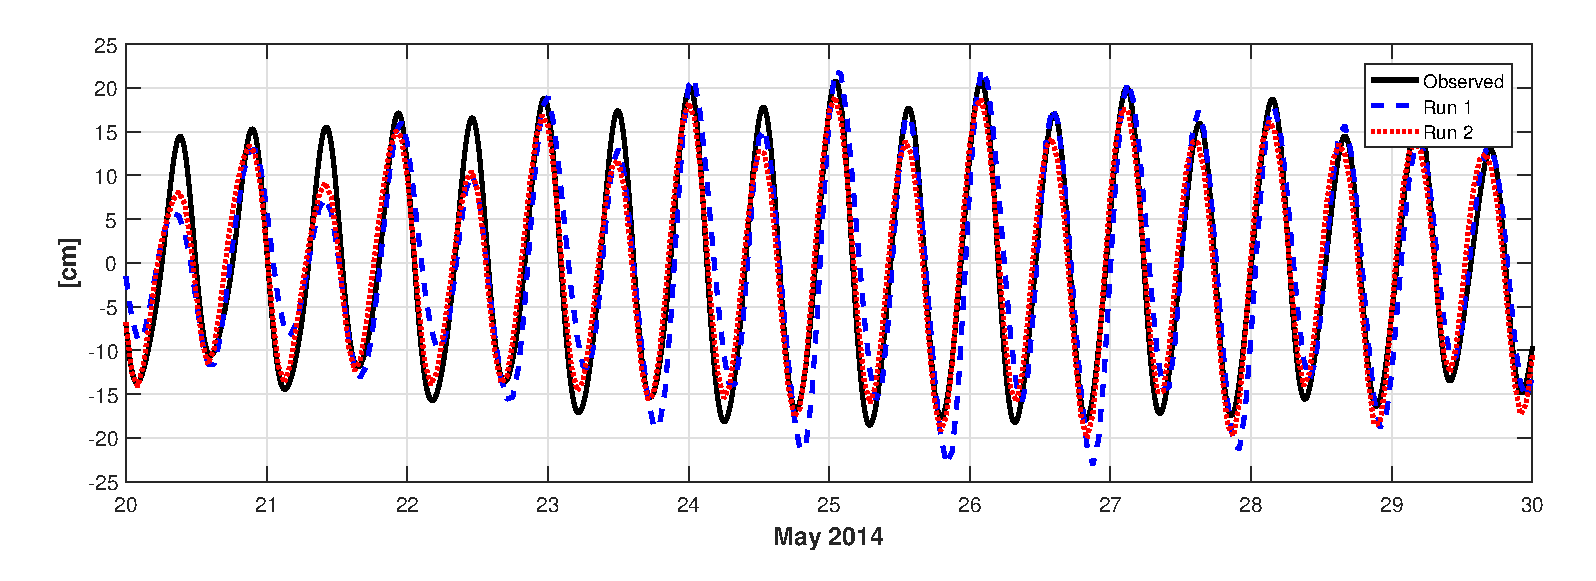
\includegraphics[width=\textwidth]{fig_Viker_timeseries}
\caption{Time series of water level at a position close to Viker in the Oslofjord}
\label{fig:Viker_timeseries}
\end{figure}



\begin{table}[ht]
%\vspace{-1.5cm}
\caption{Tidal amplitudes [cm] and phases [deg] for the water level at Viker in the Oslofjord together with adjustment factors $c^{(n)}$ and phase shifts $\triangle \phi^{(n)}$ for each component}
\label{tab:Viker}
\centering
\begin{tabular}{crrrrrrrrrr} \hline
       & Period & \multicolumn{2}{c}{Observed} & \multicolumn{2}{c}{Run 1} & \multicolumn{2}{c}{Run 2} & \multicolumn{2}{c}{Adjustment} \\
Comp.  & [h] $\;\;$ & [cm] & [deg] & [cm] & [deg] & [cm] & [deg] & $c^{(n)}$ & $\triangle \phi^{(n)}$  \\ \hline 
S$_2$  &  12.0000 &   3.0 &  39 &    5.1 &  81 &    3.2 &  67 &    0.588 &   -42.4   \\
M$_2$  &  12.4206 &  11.8 & 105 &    9.7 & 122 &   11.8 & 105 &    1.224 &   -16.8   \\
N$_2$  &  12.6584 &   3.4 &  57 &    5.7 &  81 &    3.1 &  69 &    0.595 &   -24.2   \\
K$_1$  &  23.9345 &   0.7 & 136 &    1.2 & 212 &    0.1 & 198 &    0.554 &   -75.9   \\
P$_1$  &  24.0659 &   0.5 &  66 &    1.2 & 212 &    0.1 & 198 &    0.424 &  -145.5   \\
O$_1$  &  25.8193 &   2.2 & 279 &    3.7 &  19 &    2.9 & 338 &    0.591 &   259.8   \\
MN$_4$ &   6.2692 &   0.4 & 263 &    1.0 & 141 &    0.3 &   7 &    0.368 &   122.2   \\
M$_4$  &   6.2103 &   1.2 & 275 &    0.7 &  25 &    1.1 & 354 &    1.742 &   249.2   \\
MS$_4$ &   6.1033 &   0.3 & 348 &    1.1 & 111 &    0.6 &  80 &    0.272 &   236.7   \\ \hline
\end{tabular}
\end{table}

\begin{table}[ht]
%\vspace{-1.5cm}
\caption{Tidal amplitudes [cm] and phases [deg] for the water level at Oscarsborg in the Oslofjord}
\label{tab:Oscarsborg}
\centering
\begin{tabular}{crrrrrrrrrr} \hline
      & Period & \multicolumn{2}{c}{Observed} & \multicolumn{2}{c}{Run 1} & \multicolumn{2}{c}{Run 2}  \\
Comp. & [h] $\;\;$ & [cm] & [deg] & [cm] & [deg] & [cm] & [deg]  \\ \hline 
S$_2$  & 12.0000 &  3.6 &  59  &   6.1 &  85  &  3.7 &  69.8  \\
M$_2$  & 12.4206 & 13.7 & 121  &  11.1 & 128  & 13.7 & 111.0  \\
N$_2$  & 12.6584 &  3.9 &  74  &   6.6 &  86  &  3.6 &  75.1  \\
K$_1$  & 23.9345 &  0.9 & 138  &   1.1 & 213  &  0.1 &  44.1  \\
P$_1$  & 24.0659 &  0.7 &  75  &   1.1 & 213  &  0.1 &  44.1  \\
O$_1$  & 25.8193 &  2.4 & 281  &   3.9 &  21  &  3.1 & 340.2  \\
MN$_4$ &  6.2692 &  0.6 & 308  &   2.0 & 163  &  0.5 &  29.1  \\
M$_4$  &  6.2103 &  1.7 & 319  &   1.4 &  44  &  2.0 &  14.5  \\
MS$_4$ &  6.1033 &  0.4 &  32  &   2.2 & 135  &  1.3 & 105.5  \\ \hline 
\end{tabular}
\end{table}


\begin{figure}[!t]
\centering
\includegraphics[trim=1cm 1cm 0cm 0cm,clip=true,width=0.49\textwidth]{fig_Oslofjorden_M2amp.eps}
\includegraphics[trim=1cm 1cm 0cm 0cm,clip=true,width=0.49\textwidth]{fig_Oslofjorden_M2phase.eps}
%\includegraphics[width=0.33\textwidth]{fig_Oslofjorden_M2camp.eps}
\caption{Fields of M$_2$ water level amplitude (left) and phase (right) in the Oslofjord. The corresponding observed values are indicated by coloured circles at the three permanent gauges in the area.}
\label{fig:Oslofjord_tidal_fields}
\end{figure}


\begin{figure}[!t]
\centering
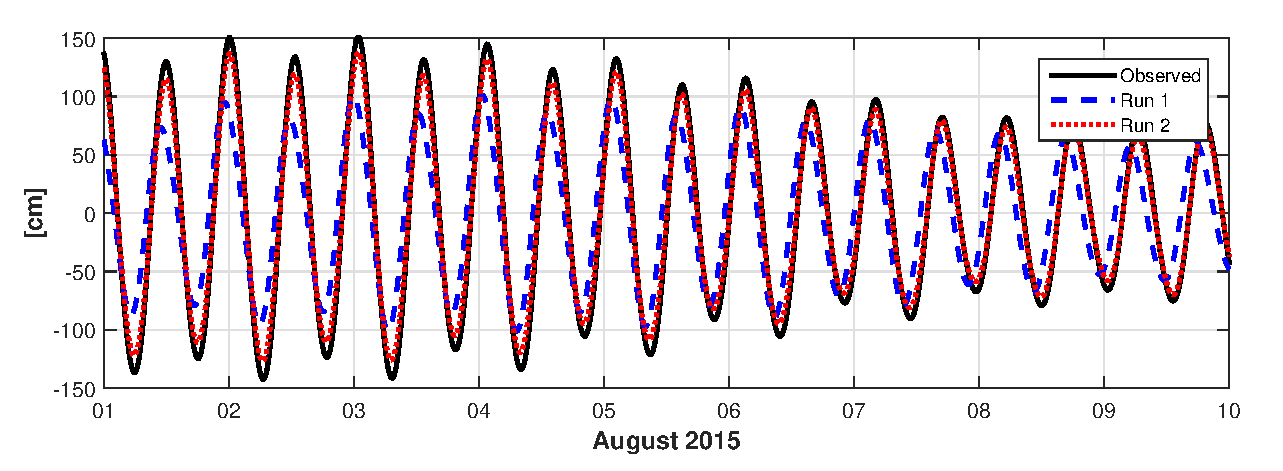
\includegraphics[width=\textwidth]{fig_Saltstraumen_timeseries}
\caption{Time series of water level at a position close to Bod{\o} in the Saltfjord}
\label{fig:Saltstraumen_timeseries}
\end{figure}


\begin{figure}[!t]
\centering
\includegraphics[width=\textwidth]{fig_Saltstraumen_M2amp}
\includegraphics[width=\textwidth]{fig_Saltstraumen_M2phase}
\caption{Fields of M$_2$ water level amplitude and phase in the Saltfjord model.}
\label{fig:Saltstraumen_field}
\end{figure}

\begin{table}[ht]
%\vspace{-1.5cm}
\caption{Tidal amplitudes [cm] and phases [deg] for the water level at Bod{\o} in the Saltfjord together with adjustment factors $c^{(n)}$ and phase shifts $\triangle \phi^{(n)}$ for each component}
\label{tab:Bodo}
\centering
\begin{tabular}{crrrrrrrrrr} \hline
      & Period & \multicolumn{2}{c}{Observed} & \multicolumn{2}{c}{Run 1} & \multicolumn{2}{c}{Run 2} & \multicolumn{2}{c}{Adjustment} \\
Comp. & [h] $\;\;$ & [cm] & [deg] & [cm] & [deg] & [cm] & [deg] & $c^{(n)}$ & $\triangle \phi^{(n)}$  \\ \hline 
S$_2$   & 12.0000  &  30.0 &      8   &  19.1 &     16   &  28.1 &      7    &   1.570  &    -7.2   \\ 
M$_2$   & 12.4206  &  87.3 &    331   &  60.0 &    301   &  78.3 &    330    &   1.454  &    29.8   \\ 
N$_2$   & 12.6584  &  18.5 &    308   &  12.7 &    271   &  16.7 &    309    &   1.461  &    37.2   \\ 
K$_1$   & 23.9345  &  10.8 &    194   &   8.8 &    183   &  10.7 &    194    &   1.225  &    11.5   \\ 
O$_1$   & 25.8193  &   3.8 &     33   &   3.3 &     39   &   3.7 &     33    &   1.154  &    -6.1   \\ 
MN$_4$  &  6.2692  &   1.5 &    229   &   0.4 &    122   &   1.5 &    228    &   3.000  &   106.9   \\ 
M$_4$   &  6.2103  &   2.7 &    268   &   3.3 &    159   &   3.1 &    283    &   0.808  &   109.5   \\ 
MS$_4$  &  6.1033  &   1.3 &      2   &   1.5 &    152   &   1.4 &     30    &   0.861  &  -149.6   \\ \hline
\end{tabular}
\end{table}


\begin{table}[ht]
%\vspace{-1.5cm}
\caption{Tidal amplitudes [cm] and phases [deg] for the water level at Finneid in the Skjerstadfjord. The observed amplitudes and phases are retrieved from The Norwegian Hydrological Survey \cite[]{tide16}.}
\label{tab:Finneid}
\centering
\begin{tabular}{crrrrrrrrrr} \hline
      & Period & \multicolumn{2}{c}{Observed} & \multicolumn{2}{c}{Run 1} & \multicolumn{2}{c}{Run 2}  \\
Comp. & [h] $\;\;$ & [cm] & [deg] & [cm] & [deg] & [cm] & [deg]  \\ \hline 
S$_2$  & 12.0000 & 15.4 &  75  &    &   &   &   \\
M$_2$  & 12.4206 & 52.9 &  25  &    &   &   &   \\
N$_2$  & 12.6584 & 10.4 &   5  &    &   &   &   \\
K$_1$  & 23.9345 &  8.0 & 235  &    &   &   &   \\
O$_1$  & 25.8193 &  2.6 &  86  &    &   &   &   \\ \hline 
\end{tabular}
\end{table}

\begin{figure}[!t]
\centering
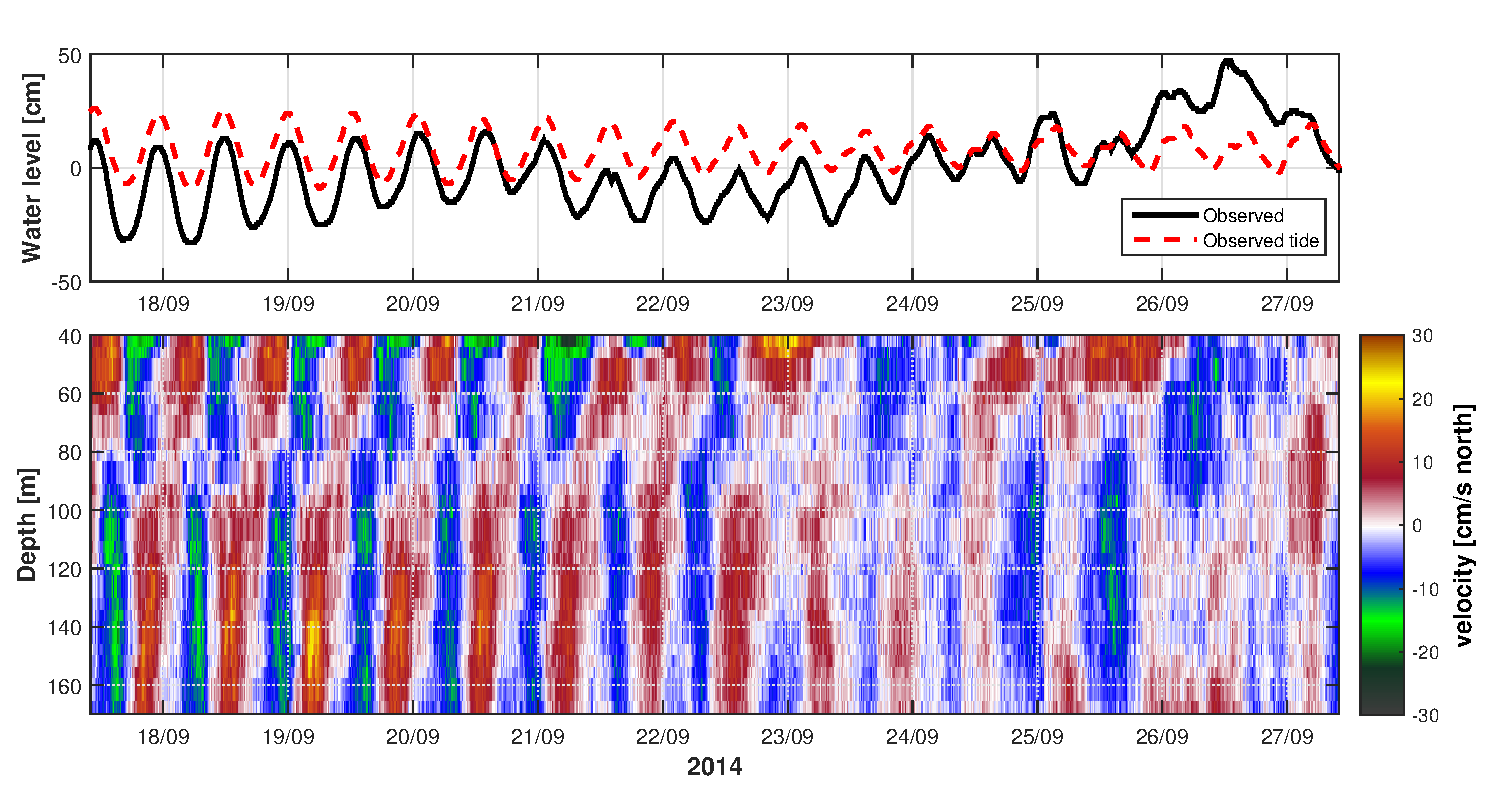
\includegraphics[width=\textwidth]{fig_Filtvedt_timeseries_obs}
\caption{Time series of water level at Oscarsborg (upper) and currents at a position close to Filtvedt (lower) in the Oslofjord. Observations at water depths less than 40 meters are not included due to noise in the upper levels.}
\label{fig:Filtvedt_timeseries_obs}
\end{figure}


\begin{figure}[!t]
\centering
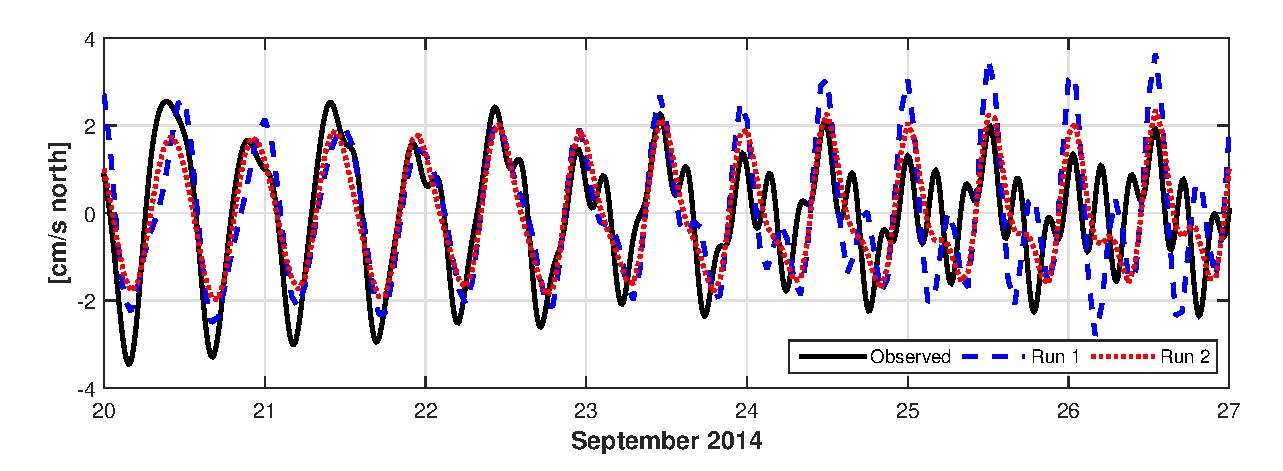
\includegraphics[width=\textwidth]{fig_Filtvedt_timeseries}
\caption{Time series of depth averaged tidal currents at a position close to Filtvedt in the Oslofjord. The time series are constructed based on the tidal components. Neither observed nor modelled currents at water depths less than 40 meters are included due to noise in the upper levels of the observations.}
\label{fig:Filtvedt_timeseries}
\end{figure}

%\begin{figure}[!t]
%\centering
%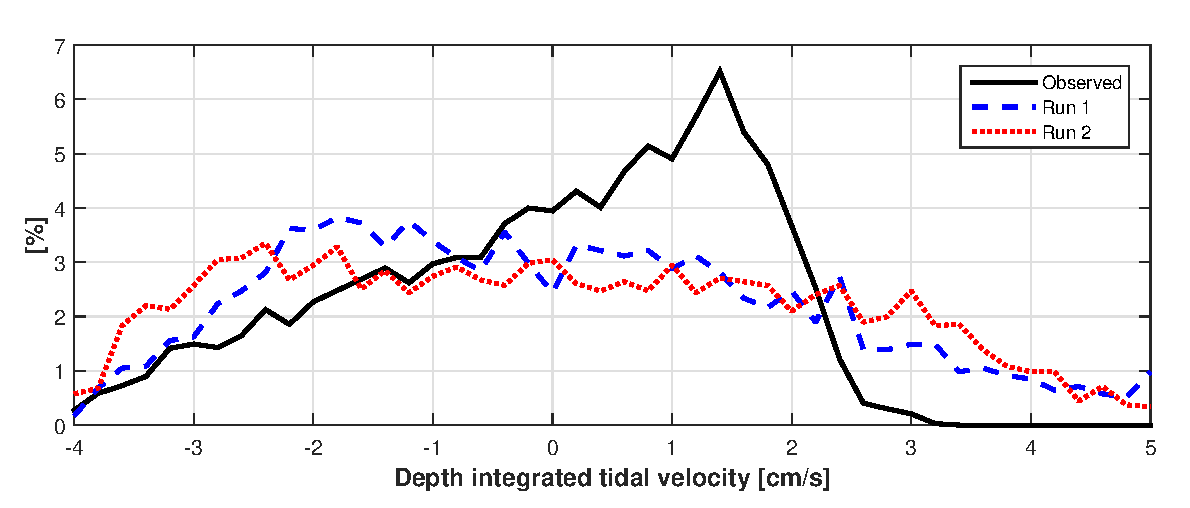
\includegraphics[width=\textwidth]{fig_Filtvedt_pdf}
%\caption{Probability density functions of observed and modelled depth integrated tidal currents at a position near Filtvedt in the Oslofjord. The bin width is here 0.1 cm/s. Only currents below 40 meters depth are included due to noise in the upper levels of the observations.}
%\label{fig:Filtvedt_pdf}
%\end{figure}


\begin{table}[ht]
%\vspace{-1.5cm}
\caption{Tidal major amplitudes [cm/s] and phases [deg] for the current near Filtvedt in the Oslofjord. The Root Mean Square Error (RMSE) for the time series of each component are computed.}
\label{tab:Filtvedt}
\centering
\begin{tabular}{crcrcrcrcc} \hline
      & Period & \multicolumn{2}{c}{Observed} & \multicolumn{2}{c}{Run 1} & \multicolumn{2}{c}{Run 2} & \multicolumn{2}{c}{RMSE} \\
Comp. & [h] $\;\;$ & [cm/s] & [deg] & [cm/s] & [deg] & [cm/s] & [deg] & Run 1 & Run 2\\ \hline 
S$_2$  & 12.0000 &  0.5 & 280  &   1.4 & 336  &  0.5 & 334  & 1.0 & 0.4 \\
M$_2$  & 12.4206 &  1.8 &   9  &   2.3 &  18  &  2.0 &  16  & 2.5 & 0.4 \\
N$_2$  & 12.6584 &  0.5 & 293  &   1.3 & 339  &  0.5 & 343  & 0.9 & 0.2 \\
K$_1$  & 23.9345 &  0.5 &  61  &   0.1 &   5  &  0.0 & 261  & 0.3 & 0.3 \\
%P$_1$  & 24.0659 &  -   &  -   &    -  &  -   &   -  &  -   \\
O$_1$  & 25.8193 &  0.1 & 120  &   0.3 & 244  &  0.2 & 250  & 0.2 & 0.1 \\
MN$_4$ &  6.2692 &  0.3 & 166  &   0.7 &  52  &  0.2 & 305  & 0.4 & 0.3 \\
M$_4$  &  6.2103 &  0.7 & 220  &   0.6 & 303  &  0.7 & 291  & 0.7 & 0.7 \\
MS$_4$ &  6.1033 &  0.0 & 252  &   0.8 &  24  &  0.4 &  19  & 0.6 & 0.2 \\
\hline 
\end{tabular}
\end{table}

